% Notes on the theory and implementation of a void correction

\documentclass[12pt]{article}
\usepackage{amsmath,amsthm,enumitem,amssymb,graphicx,color,bm}
\usepackage[margin=1in]{geometry}

\makeatletter
\def\imod#1{\allowbreak\mkern10mu({\operator@font mod}\,\,#1)}
\makeatother

\begin{document}

\setlength\parindent{0pt}

\vspace{-6in}

\title{Void Correction Notes}
\author{Spencer Everett}
\date{\today}

\maketitle

\section*{Motivation}

The shear and convergence predictions made by the \texttt{Pangloss} framework are dependent upon the cosmology assumed; inherent in all distance calculations are the value and evolution of the universe's mass density, characterized by $\Omega_m(z)$. Yet the current framework overestimates the mass in all regions as it adds the halo masses on top of a uniformly distributed mass density that is already equal to the predicted mass density at the halos' respective redshifts. Even more problematic, much of the mass in the Millennium Simulation isn't contained in halos - and the weak lensing contributions of these mass structures are not currently accounted for.\\

To have a more accurate approximation for the mass density in a given region (and thus more accurate $\gamma$ and $\kappa$ predictions), we must account for mass in \texttt{Pangloss} in three different components:

\begin{enumerate}[label=(\arabic*)]
\item The mass contributed by galaxies (stellar mass), halos, and subhalos,
\item A ``foreground correction'' in the form of a uniformly distributed sheet of negative mass density at each redshift such that the mean density (and thus mean $\kappa$) of the redshift slice is zero, and
\item A ``smooth component correction'' in the form of a uniformly distributed sheet of mass density at each redshift that accounts for all excess mass in the region not contained in galaxies or their halos (i.e. cluster and supercluster halos, filaments, etc.)
\end{enumerate}

The first component is accounted for when calculating $\kappa$ predictions in \texttt{makeKappas()} that is called by \texttt{lens\_by\_halos()}, although we currently ignore the stellar and subhalo masses as they are less significant. We can calculate the other two components in the following ways:

\begin{enumerate}[label=(\arabic*)]
\setcounter{enumi}{1}
\item To start, we can make the foreground correction on each foreground catalog separately by snapping the entire catalog to the same redshift grid that the lightcone halos eventually will use. The surface mass density as a function of redshift then can be calculated by summing the mass in (1) and dividing by the proper surface area at each redshift. This surface mass density is used to calculate the $\kappa$ contribution corresponding to the entire foreground at that redshift.
\item If we derive equations for the universe's mass density and halo mass density in our lightcones as a function of redshisft, then the smooth-component correction at each redshift should simply be the difference between these two densities. Calculating the halo mass density will require an expression for the proper volume element and integrating over each redshift slice.
\end{enumerate}

We now derive each correction below.

\section*{The Foreground Correction}

(Details to be added later!)

\section*{The Smooth-Component Correction}

The foreground catalogs of the Millennium Simulation contain only the stellar masses of foreground galaxies and the masses of their respective dark matter halos and subhalos; all additional mass in the form of filaments, galaxy cluster and supercluster halos, or otherwise must be inferred. However, the mean mass density of large enough ($\sim$100 Mpc) regions should approximate the mean mass density of the universe, so for a first guess we can approximate the additional mass as a series of uniform sheets of matter along each redshift slice that make the total mass density of the foreground catalog equal to the mean density of the universe. This assumption can be expressed as

\begin{equation}\label{smooth_correction1}
\rho_{\text{matter}}(z)=\rho_{\text{halos}}(z)+\rho_{\text{smooth}}(z)
\end{equation}

where $z$ is the redshift and $\rho_{\text{matter}}(z)$, $\rho_{\text{halos}}(z)$, and $\rho_{\text{smooth}}(z)$ are the mean matter densities of the universe, halos, and smooth-component correction respectively. For simplicity, we rename theses quantities ${\rho_m(z)}$, ${\rho_h(z)}$, and ${\rho_s(z)}$ so that Equation \eqref{smooth_correction1} now reads as

\begin{equation}\label{smooth_correction2}
\rho_m(z)=\rho_h(z)+\rho_s(z).
\end{equation}

To solve for the desired smooth component correction, we first need to calcualte ${\rho_m(z)}$ and ${\rho_h(z)}$ and then subtract:

\begin{equation}\label{smooth_correction2}
\rho_s(z)=\rho_m(z)-\rho_h(z).
\end{equation}

Note that, unlike the foreground correction, each mass sheet at a given $z$ can have positive \textit{or} negative mass density as the foreground at that redshift could happen to be in a local overdensity or underdensity.

\subsection*{Calculating $\bm{\rho_m(z)}$:}

Using the fluid equation and equation of state, we can show that the energy density of non-relativistic matter $\varepsilon_m(z)$ evolves as

\begin{equation}\label{energy_evol}
\varepsilon_m(z)=\frac{\varepsilon_{m,0}}{a(z)^3}=\varepsilon_{m,0}(1+z)^3
\end{equation}

where $a(z)=(1+z)^{-1}$ is the cosmic scale factor ($a(0)=1$ by convention) and a subscript of 0 means the value at the present time, or equivalently a redshift of 0. \textcolor{red}{(Maybe show the full derivation in the thesis?)} This makes sense as the (mostly constant) mass is being diluted by an expanding volume. As the mass is non-relativistic, its energy density can be approximated by

\begin{equation*}\label{energy_mass}
\varepsilon_m(z)\approx\rho_m(z)c^2
\end{equation*}

and thus

\begin{equation}\label{mass_evol}
\rho_m(z)\approx\rho_{m,0}(1+z)^3.
\end{equation}

The current matter density $\rho_{m,0}$ is usually reported in literature in terms of the present matter density parameter $\Omega_{m,0}$ defined as

\begin{equation}\label{}
\Omega_{m,0}=\frac{\rho_{m,0}}{\rho_{c,0}}=\frac{8\pi G}{3H_0^2}\,\rho_{m,0}
\end{equation}

where $\rho_{c,0}=\frac{3H_0^2}{8\pi G}$ is the present critical density. Solving for $\rho_{m,0}$ gives

\begin{equation*}\label{}
\rho_{m,0}=\frac{3H_0^2}{8\pi G}\,\Omega_{m,0}
\end{equation*}

and so we may write the non-relativistic mass density of the universe as a function of redshift as

\begin{equation}\label{rho}
\rho_m(z)\approx\left(\frac{3H_0^2}{8\pi G}\,\Omega_{m,0}\right)(1+z)^3.
\end{equation}

Current \texttt{Pangloss} code assumes a cosmology of $\Omega_{m,0}=0.25$, $\Omega_{\Lambda,0}=0.75$ (to ensure a flat universe), and $H_0=73$ km$\cdot$s$^{-1}\cdot$Mpc$^{-1}$ (\textcolor{red}{Were these values chosen to match the original Millennium Simulation parameters? A later run that Stefan used for his ray tracing? Known values when Collett et al. was published?}) which leads to an evolving mass density of

\begin{equation}\label{rho}
\rho_m(z)\approx\left(3.70\times10^{10}\frac{M_{\odot}}{\text{Mpc}^3}\right)(1+z)^3.
\end{equation}

\subsection*{Calculating $\bm{\rho_h(z)}$:}

Now we must calculate $\rho_h(z)$ given the foreground catalogs of the Millennium Simulation. While each galaxy/halo are on a continuum of redshifts, we snap each halo to one of $N$ redshift planes from $z=0$ to the source redshift of $z_s=1.3857$, each separated by a constant $\Delta z=1.3857/N$ for faster computation (typically, $N=100$ and $\Delta z\approx0.014$). We can approximate $\rho_h$ at each of the $N$ redshift values by summing the halo masses and dividing by the integral the proper volume element $dV_p$ over the redshift range $z\pm \Delta z/2$ and solid angle $d\Omega$ covered by the foreground catalog. Figure \ref{rho_slice} visualizes this process.\\

\begin{figure}[!ht]
  \centering
  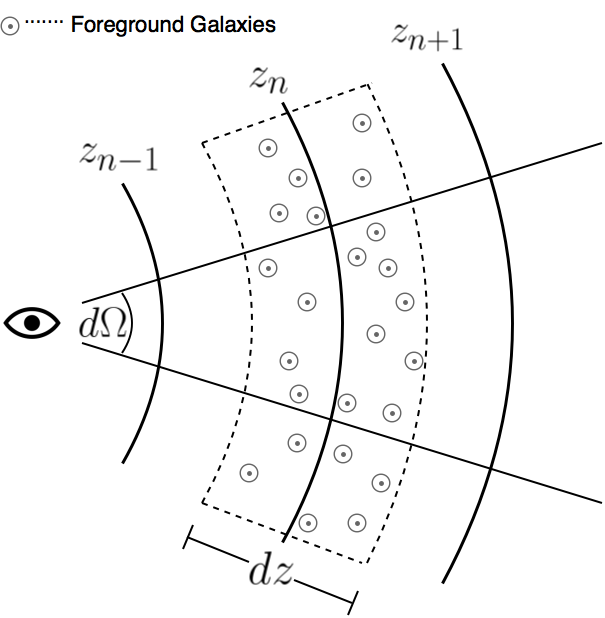
\includegraphics[width=0.6\textwidth]{figs-swe/comoving_integral.png}
  \caption{Approximating $\rho_h(z)$ by summing the halo mass in each redshift slice and dividing by the proper volume. Each slice covers a redshift range of $\Delta z$ (except for $z=0$ and $z=1.3857$, which have a range of $\Delta z/2$) and solid angle $d\Omega$.}
  \label{rho_slice}
\end{figure}

From Figure \ref{rho_slice}, it is clear that we want a proper volume element that is expressed in terms of the solid angle $d\Omega$ (or really, $d\theta d\phi$) and the redshift $dz$. To do this, we can start with the standard spherical volume element $dV=r^2\sin(\theta)drd\theta d\phi$. However, we must be careful that (1) we are using proper distances, (2) account for the possibility of a curved universe, and (3) use the correct distance measure for $r$ (in this case, the angular diameter distance). From this we can gather that the proper volume element must have the form of

\begin{equation}\label{proper_element}
dV_p=dr_pdA=d_A(z)^2dr_pd\omega=d_A(z)^2\sin(\theta)dr_pd\theta d\phi
\end{equation}
% and $r_a$ is the angular diameter distance 
where $d_A(z)$ is the angular diameter distance and the subscript $p$ denotes proper distance. When the angular diameter distance $d_A(z)$ is multiplied by an angle (i.e. $d_A(z)d\theta$ and $d_A(z)d\phi$), it gives an approximation of the proper distance between two objects at the same redshift. $d_A(z)$ can be expressed in terms of the transverse comoving distance $d_M(z)$,

\begin{equation}\label{angular2transverse}
d_A(z)=a(z)d_M(z)=\frac{d_M(z)}{1+z}
\end{equation}

which is the comoving analog of $d_A(z)$. The transverse comoving distance depends on the assumed cosmology of the universe and takes the form of

\begin{equation}\label{comoving_transverse}
d_M(z)=\left\{
     \begin{array}{lr}
       d_H/\sqrt{\Omega_k}\sinh\left[\sqrt{\Omega_k}d_C(z)/d_H\right] & : \Omega_k>0\\
       d_C(z) & : \Omega_k=0\\
       d_H/\sqrt{|\Omega_k|}\sin\left[\sqrt{|\Omega_k|}d_C(z)/d_H\right] & : \Omega_k<0
     \end{array}
   \right.
\end{equation}

where $d_H=c/H_0$ is the Hubble distance, $\Omega_k$ is the curvature parameter ($\Omega_k=0$ for a flat universe), and $d_C(z)$ is the line-of-sight (LOS) comoving distance given by

\begin{equation}\label{comoving_distance}
d_C(z)=d_H\int_0^z\frac{dz^\prime}{E(z^\prime)}
\end{equation}

where $E(z)$ is the dimensionless Hubble parameter

\begin{equation}\label{dim_hubble_parameter}
E(z)=\sqrt{\Omega_m(1+z)^3+\Omega_k(1+z)^2+\Omega_\Lambda}.
\end{equation}

Substituting Equation \eqref{angular2transverse} into \eqref{proper_element} leads to

\begin{equation}\label{temp_solution}
dV_p=d_a(z)^2\sin(\theta)dr_pd\theta d\phi=\left(\frac{d_m(z)}{(1+z)}\right)^2\sin(\theta)dr_pd\theta d\phi=\frac{d_m(z)^2\sin(\theta)}{(1+z)^2}dr_pd\theta d\phi
\end{equation}

and so all that remains is to express $dr_p$ in terms of $dz$. As the LOS proper distance between two objects $r_p(z)$ is related to the LOS comoving distance $d_C(z)$ by

\begin{equation}\label{physical2comoving}
r_p(z)=a(z)d_C(z)=\frac{d_C(z)}{1+z}=\frac{d_H}{1+z}\int_0^z\frac{dz^\prime}{E(z^\prime)},
\end{equation}

it follows that that an infinitesimal proper displacement $dr_p$ is given by

\begin{equation}\label{physical2comoving_inf}
dr_p=\frac{d_H}{E(z)(1+z)}dz.
\end{equation}

Combining this result with Equation \eqref{temp_solution} leads to the desired proper volume element given by

\begin{align}
dV_p&=\frac{d_m(z)^2\sin(\theta)}{(1+z)^2}dr_pd\theta d\phi\nonumber\\
&=\frac{d_m(z)^2\sin(\theta)}{(1+z)^2}\left(\frac{d_H}{E(z)(1+z)}dz\right)d\theta d\phi\nonumber\\
&=\frac{d_Hd_M(z)^2\sin(\theta)}{E(z)(1+z)^3}dzd\theta d\phi.
\end{align}

We can calculate the proper volume of a given grid slice at redshift $z$ in a foreground catalog centered at ($\theta,\phi$) by integrating the above volume element over the $\Delta z$, $\Delta\theta$, and $\Delta\phi$ range of the redshift slice:

\begin{equation}
V(z)=\int_{V_z}dV_p=d_H\int_{z-\frac{\Delta z}{2}}^{z+\frac{\Delta z}{2}}\int_{\theta-\frac{\Delta\theta}{2}}^{\theta+\frac{\Delta\theta}{2}}\int_{\phi-\frac{\Delta\phi}{2}}^{\phi+\frac{\Delta\phi}{2}} \frac{d_M(z^\prime)^2\sin(\theta^\prime)}{E(z^\prime)(1+z^\prime)^3}dz^\prime d\theta^\prime d\phi^\prime.
\end{equation}

Integrating over $d\theta^\prime$ and $d\phi^\prime$ and using the trig identity ${\cos(u)-\cos(v)=2\sin\left(\frac{u+v}{2}\right)\sin\left(\frac{u-v}{2}\right)}$ gives

\begin{equation}\label{volume_final}
V(z)=2d_H\Delta\phi\sin(\theta)\sin(\Delta\theta/2)\int_{z-\frac{\Delta z}{2}}^{z+\frac{\Delta z}{2}} \frac{d_M(z^\prime)^2\sin(\theta^\prime)}{E(z^\prime)(1+z^\prime)^3}dz^\prime d\theta^\prime d\phi^\prime
\end{equation}

which is our final expression for the proper volume.\\

With the proper volume calculated, the halo mass density $\rho_h(z)$ is simply the sum of the individual halo masses $M_{i,z}$ in the $z$-plane divided by Equation \eqref{volume_final}:

\begin{equation}\label{rho_h}
\rho_h(z)=\frac{\sum_i M_{i,z}}{V(z)}=\frac{\sum_i M_{i,z}}{2d_H\Delta\phi\sin(\theta)\sin(\Delta\theta/2)\int_{z-\frac{\Delta z}{2}}^{z+\frac{\Delta z}{2}} \frac{d_M(z^\prime)^2\sin(\theta^\prime)}{E(z^\prime)(1+z^\prime)^3}dz^\prime d\theta^\prime d\phi^\prime}.
\end{equation}

\subsection*{Calculating $\bm{\rho_s(z)}$:}

Now that $\rho_m(z)$ and $\rho_h(z)$ have been calculated, the smooth-component correction $\rho_s(z)$ is simply the difference between the two:

\begin{align}\label{smooth_component} 
\rho_s(z)&=\rho_m(z)-\rho_h(z)\nonumber\\
&=\left(\frac{3H_0^2}{8\pi G}\,\Omega_{m,0}\right)(1+z)^3 - \frac{\sum_i M_{i,z}}{2d_H\Delta\phi\sin(\theta)\sin(\Delta\theta/2)\int_{z-\frac{\Delta z}{2}}^{z+\frac{\Delta z}{2}} \frac{d_M(z^\prime)^2\sin(\theta^\prime)}{E(z^\prime)(1+z^\prime)^3}dz^\prime d\theta^\prime d\phi^\prime}
\end{align}

where $\rho_s(z)$ is a discrete function only evaluated at the $N$ values of $z$. Finally, note that this equation needs a small correction in the integral bounds for the boundary cases of $z=0$ and $z=1.3857$. Simply change the bounds to ($0,\Delta z$) and ($z-\Delta z,z$) respectively.

\end{document}

% Assumptions: only slow moving (not just non-relativistic!) mass, all extra matter in a sheet, same sigma_crit for the whole plane, 
